%
% hardware.tex
%
% Copyright (C) 2020 by SpaceLab.
%
% Flatsat Platform Documentation
%
% This work is licensed under the Creative Commons Attribution-ShareAlike 4.0
% International License. To view a copy of this license,
% visit http://creativecommons.org/licenses/by-sa/4.0/.
%

%
% \brief Hardware chapter.
%
% \authors: Gabriel Mariano Marcelino <gabriel.marcelino@spacelab.ufsc.br> and Yan Castro de Azeredo <yan.azeredo@spacelab.ufsc.br>
%
% \institution Universidade Federal de Santa Catarina (UFSC)
%
% \version 0.1.1
%
% \date 2020/10/11
%

\chapter{Hardware} \label{ch:hardware}

This chapter describes all the FlatSat's hardware interfaces in detail. On figures \ref{fig:pcb-top} and \ref{fig:pcb-bottom} are displayed de top and bottom PCB prints.

\section{PC104 Interfaces}

On SpaceLab's FlatSat Platform the PC104 interfaces are composed by two 52 pins with 2.54mm pitch connectors. Slots Nº2 to Nº7 has two \textit{SSW-126-01-G-D} and the slot Nº1 uses two \textit{TSW-126-07-G-D} connectors with inverted pinout, see figures \ref{fig:flatsat-top-view} and \ref{fig:flatsat-n1-slot}. All pins are interconected to flexiblesize the positioning of the modules. All slots have labeled MEC\# grounded mouting holes for modules.

\section{Binding Posts and Power Receptacles}

Two sets of binding posts (\textit{4243-0}) can be mouted on the PCB to be used for two external power supplies, see figure \ref{fig:binding-posts}. The modules are powered via external jumper wires to the 12 position receptacle connectors (\textit{BCS-106-L-D-TE}). The labeled '+' pins are the positive power while the labeled '-' pins are GND, see figure \ref{fig:power-receptacles}.

\section{Charge Header}

On the board there is a JST XH 2 position header (\textit{B2B-XH-A-M(LF)(SN)}) for charging batteries, it can be seen in figure \ref{fig:charge-header}. The component can suport up to 3000mA of current, but it is advised to be used with less than 1500mA. The 4 pin PicoBlade connector showed in figure \ref{fig:charge-picoblade} is to be connected to the EPS module to make the interconnection for the JST header. The charge header also provides a detent lock for fastening and avoid a mistankenly reverse connection.

\section{RBF Pin Header}

The platform has a Remove Before Flight (RBF) pin header that can seen figure \ref{fig:rbf-pin-header}. The interconnection between the header and the EPS module is done by a 4 pin PicoBlade, also seen on figure \ref{fig:rbf-pin-header} labeled "CN9".

\section {SPDT Kill-Switches}

The kill-switches uses SPDT switches (\textit{100SP1T1B4M2QE}) for powering off the EPS module, see figure \ref{fig:kill-switches-spdts}. The power off states are seen on figure \ref{fig:kill-switches-operation}, they are also present on the hardware schematics. The SPDTs are interconnected to the EPS module via two 6 pin PicoBlade connectors, labeled "CN1" and "CN8", also showed in figure \ref{fig:kill-switches-spdts}.

\section{Antenna Interfaces}

\subsection{SMA connectors}

On the PCB there are SMA connectors (\textit{132134-15}) labeled "ANT1" to "ANT8" for connecting VHF, UHF and S band antennas. The receiver (Rx) antenna is to be connected to one of the SMA, while the transmitter (Tx) goes to the other connector and to the CubeSat modules. The impedance control (see figure \ref{fig:rf-track-width-calc}) and power dissipation (see figure \ref{fig:rf-track-width-power-calc}) where approximately calculated for all 3 bands. As the FlatSat platform is to be used in light testing the aproximations where considered acceptable for the project.

\subsection{Impedance Control of the RF Tracks}

\begin{figure}[!ht]
    \begin{center}
        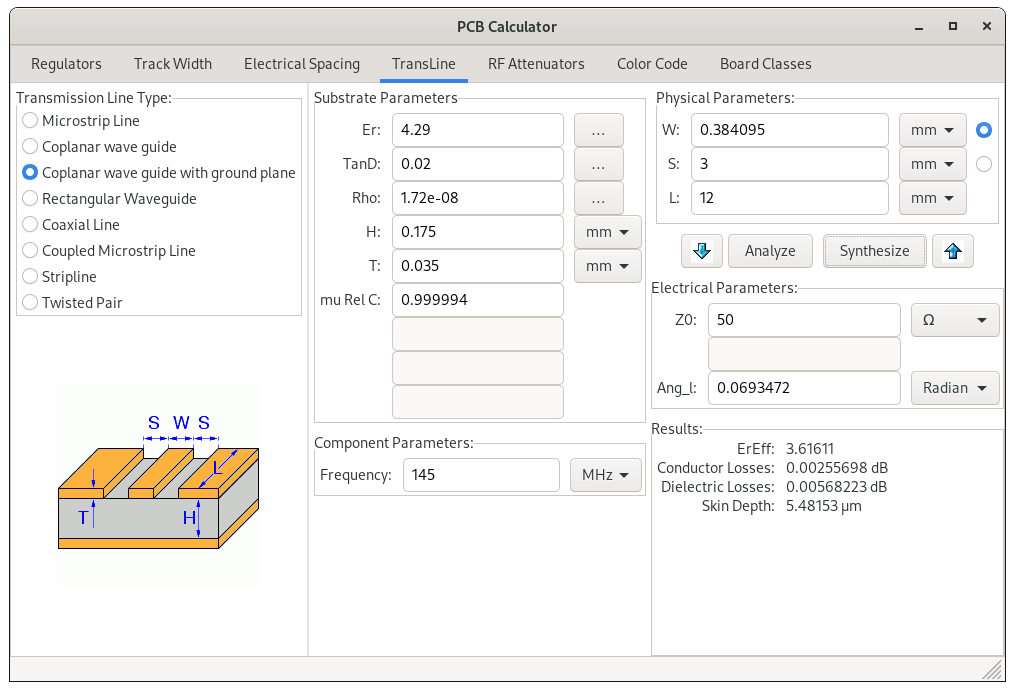
\includegraphics[width=\textwidth]{figures/rf-track-width}
        \label{fig:rf-track-width-calc}
        \caption{Calculation of the width of the RF tracks.}
    \end{center}
\end{figure}

\begin{figure}[!ht]
    \begin{center}
        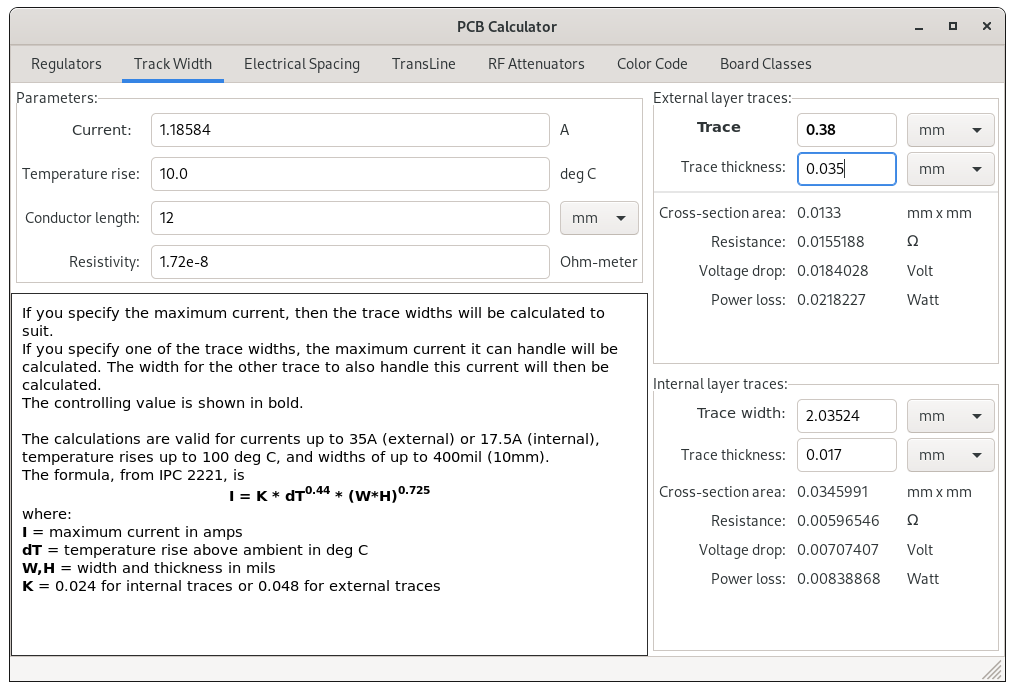
\includegraphics[width=\textwidth]{figures/rf-track-width-power}
        \label{fig:rf-track-width-power-calc}
        \caption{Power dissipation of the RF tracks.}
    \end{center}
\end{figure}

\section{UART to USB Converter}

There is a UART to USB converter circuit built-in the FlatSat platform for debbuging pourposes for four independent modules, it can be seen on figure \ref{fig:ft4232h-circuit}. The subcircuit is self powered from a USB cable connecting a computer to a micro USB type B port (\textit{10118194-0001LF}). The    
USB Bridge converter IC is the \textit{FT4232HL-REEL} from FTDI. PicoBlade connectors are used for connecting the IC to the modules, see figures \ref{fig:uart-picoblades}. It is also possible to use jumper wires connecting the 12 Position receptacle connector (\textit{BCS-106-L-D-TE}) to the modules if PicoBlades are not used, see figure \ref{fig:uart-receptacle}.